\chapter{Results}
\label{chap:results}
\section{Ciphertext Visualisations}
In order to visually demonstrate the encryption, visualisations of the ciphertext polynomial $c_0$ (refer to \cref{sec:ckks}) were generated using a \gls{crt} decomposition of the \gls{rns} representation of $c_0$.
Each pixel corresponds to a coefficient $a \in \Z / q\Z$ scaled down by the modulus $q$ to obtain a brightness value between $0$ and $1$.

\begin{figure}[H]
  \centering
  % 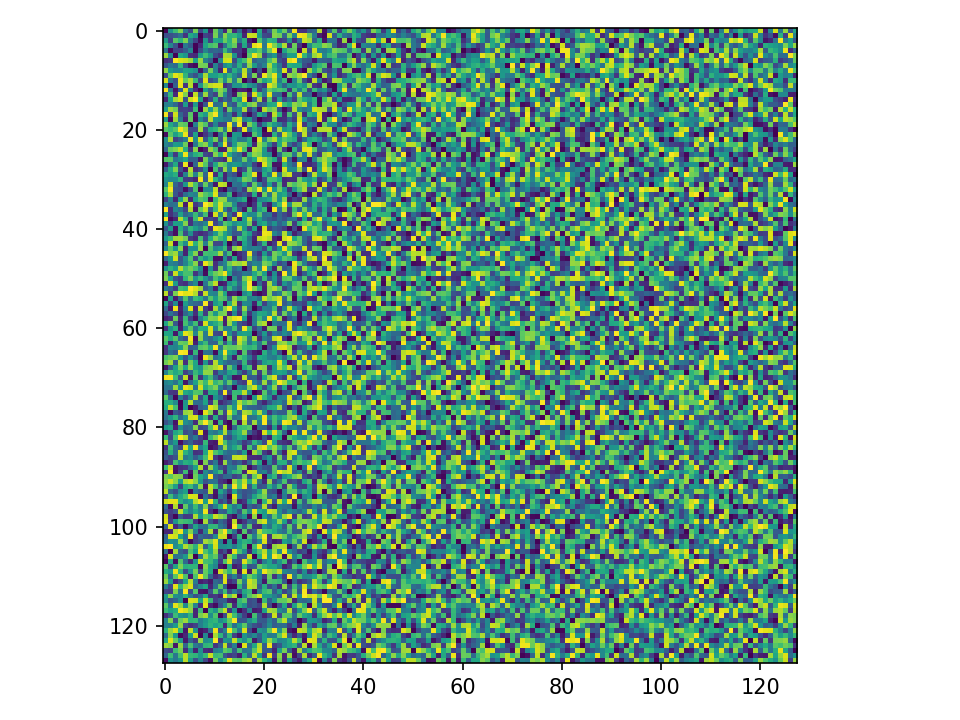
\includegraphics[width=\linewidth]{figures/ciphertext-visualisation.png}
  \inputtikz{figures/ciphertext-visualisation}
  \caption[Visualisation of the plain input images compared to their ciphertext]{Ciphertext Visualisation: The first row corresponds to the images in plain, the second row depicts an encrypted version, namely the reconstructed polynomial coefficients $a_k$ of the ciphertext polynomial.}
  \label{fig:ciphertext-visualisation}
\end{figure}

\section{The Training Process}
\begin{figure}[H]
  \centering
  \pgfplotsset{/pgfplots/group/.cd,vertical sep=1.6cm}
  \inputtikz{figures/generated/training-history}
  \caption[Classification accuracy and loss development during training]{
    Development of the classification accuracy and the mean squared error during the training process of our neural network.
    Training and validation set metrics are plotted separately.
    When the validation accuracy starts to drop, the training process halts with the next epoch to prevent overfitting.
  }
  \label{fig:training-history}
\end{figure}

The machine learning framework behind the project, Tensorflow, splits its training process into \textit{epochs}, which can be found on the x-axis in the plot above.
For each training epoch, we find the progress that has been made in a single epoch by looking at the new accuracy (which percentage of the images has been classified correctly) and the loss function (\gls{mse} in this case).
Per training run, we make a differentiation between training metrics and validation metrics, illustratively shown above for the given network.
The validation data is not involved with the training process, it is only used to find a point in the process when training accuracy still rises while validation accuracy starts to drop (confer \cref{fig:training-history}).
At this point we will likely find the network's learning process in an \textit{overfitting} situation, so the training process terminates.

\section{Accuracy, Precision, Recall}
\label{sec:accuracy-precision-recall}
\begin{figure}[H]
  \centering
  \inputtikz{figures/generated/confusion-matrix}
  \caption[Confusion Matrix of the trained network]{
    The Confusion Matrix of the trained network, showing digit-wise correct classifications in the diagonal and misclassifications, per digit-pair, in the off-diagonals.
    The matrix values were visually enhanced by mapping them to their logarithm base 2.
  }
  \label{fig:confusion-matrix}
\end{figure}

As we can see in \cref{fig:confusion-matrix}, the majority of all images are classified correctly (visible in the diagonal).
What makes the confusion matrix so interesting is identifying frequently mixed up digits - for instance, 3 and 5, 2 and 7 or 4 and 9.
Judging with a human eye, this is somewhat reasonable - even more so when looking at the actual set of misclassified images (\cref{fig:misclassifications}).

\begin{figure}[H]
  \centering
  \inputtikz{figures/misclassifications}
  \caption[Misclassified images of the test set]{
    \gls{mnist} test images with true labels $0, 1, 2, 3, 4, 5, 6, 7, 8, 9$ that were misclassified as $6, 8, 9, 8, 2, 6, 0, 9, 2, 3$ by the neural network.
  }
  \label{fig:misclassifications}
\end{figure}

The plain network classifies \SI{97.62}{\percent} of the 10,000 test images correctly.
Running the encrypted classification on the full test set too, the encrypted network classifies \SI{97.31}{\percent} of the test images correctly in $3\frac{1}{2}$ hours at full CPU utilisation, using the hybrid matrix multiplication method.
For a binary classification, two further metrics of interest are
$$\text{Precision} = \frac{\text{tp}}{\text{tp} + \text{fp}} \quad\quad
  \text{Recall} = \frac{\text{tp}}{\text{tp} + \text{fn}}$$

with
$\text{tp}$ ... True Positives,
$\text{fp}$ ... False Positives,
$\text{fn}$ ... False Negatives.

Precision (also referred to as PPV, positive predictive value) refers to the ability of the network to classify positive samples correctly, while Recall explains the completeness of the classified samples (i.e. how few true positives have been left out).

\begin{table}[H]
  \centering
  \caption[Precision and recall of each digit]{Precision and Recall of the trained network for each digit individually, above for the plain network evaluation (P) and below for the encrypted evaluation (E).}
  \begin{tblr}{r|cccccccccc}
    \textbf{Digit}     & 0     & 1     & 2     & 3     & 4     & 5     & 6     & 7     & 8     & 9     \\
    \hline
    \textbf{Precision (P)} & 0.978 & 0.990 & 0.959 & 0.960 & 0.985 & 0.968 & 0.977 & 0.976 & 0.963 & 0.978 \\
    \textbf{Recall (P)}    & 0.986 & 0.989 & 0.975 & 0.977 & 0.975 & 0.964 & 0.980 & 0.964 & 0.967 & 0.955 \\
    \hline
    \textbf{Precision (E)} & 0.987 & 0.976 & 0.979 & 0.946 & 0.961 & 0.960 & 0.981 & 0.974 & 0.975 & 0.956 \\
    \textbf{Recall (E)}    & 0.989 & 0.990 & 0.958 & 0.981 & 0.975 & 0.966 & 0.972 & 0.963 & 0.937 & 0.959 \\
  \end{tblr}
\end{table}

Averaged over all digits, the mean precision amounts to \SI{97.37}{\percent} while the average recall is similarly high at \SI{97.36}{\percent}.
The encrypted network evaluation yields an average Mean Max-Relative Error (see \cref{tab:performance-benchmarks}) of \SI{2.97}{\percent} using the hybrid method.

\section{Performance Benchmarks}
\label{sec:performance-benchmarks}
This section focusses on runtime and communication overhead analysis.
For fair comparisons, the preparations required for each method individually were not taken into account, as they can be performed once at the beginning of the program.

\vspace{6pt}
\begin{table}[H]
  \centering
  \caption[Performance Benchmarks / Communication Overhead]{
    Performance benchmarks and communication overhead of the classification procedure on an Intel\textregistered \, i7-5600U CPU, including the encoding and decoding steps.
    Different parameter sets $\bm{B_1}, \bm{B_2}, \bm{N}$ are compared for each of the implemented matrix multiplication methods \textit{diagonal}, \textit{hybrid} and \textit{Babystep-Giantstep} (\glstext{bsgs}), looking at the averaged runtime, message size and also the accuracy when compared to the plain result ($\bm{\Delta}$).
    \vspace{6pt}
  }
  \caption*{
    $\bm{B_1}$ ... Coefficient Moduli start bits (also equal to the last) \\
    $\bm{B_2}$ ... Coefficient Moduli middle bits, also defines the scale as $2^{B_2}$ \\
    $\bm{N}$ ... Polynomial Modulus Degree, found in the exponent of $p(X) = X^N + 1$ \\
    $\bm{T}$ ... Runtime of encryption + classification + decryption \\
    $\bm{M}$ ... Message Size (Relin Keys + Galois Keys + Request Ciphertext + Response Ciphertext) \\
    $\bm{\Delta}$ ... Mean Max-Relative Error compared to the exact result, i.e. $\frac{\langle |\bm{y}_{prediction} - \bm{y}_{exact}| \rangle}{\max |\bm{y}_{exact}|}$
  }
  \SetTblrInner{rowsep=1pt}
  \begin{tblr}{
    colspec={ccrrrrrrr},
    row{2,3,4} = {bg=azure9},
    row{5,6,7} = {bg=violet9},
    row{8,9,10} = {bg=blue9},
    row{11,12,13} = {bg=azure9},
        % row{14,15,16} = {bg=azure9},
        % row{2,5,8,11,14,17} = {abovesep=4pt},
        % row{4,7,10,13,16,19} = {belowsep=4pt},
      }
    \hline
    \bf Mode & \bf SecLevel & $\bm{B_1}$ & $\bm{B_2}$ & $\bm{N}$ & \bf MatMul & $\bm{T}$ / \si{\second} & $\bm{M}$ / \si{\mebi\byte} & $\bm{\Delta}$ / 1 \\
    \hline
    Release & tc128 & 34 & 25 & 8192 & Diagonal & 8.39623 & 132.72 & 0.036462 \\
    &&&&& Hybrid & 1.35514 & 132.72 & 0.0362841 \\
    &&&&& BSGS & 1.66998 & 132.72 & 0.143365 \\
    \hline
    & tc128 & 60 & 40 & 16384 & Diagonal & 17.2416 & 286.508 & 0.0363667 \\
    &&&&& Hybrid & 3.05702 & 286.508 & 0.0364073 \\
    &&&&& BSGS & 3.66647 & 286.508 & 0.139999 \\
    \hline
    & tc256 & 60 & 40 & 32768 & Diagonal & 35.2401 & 615.163 & 0.036366 \\
    &&&&& Hybrid & 5.99692 & 615.163 & 0.0364071 \\
    &&&&& BSGS & 7.34914 & 615.163 & 0.139999 \\
    \hline
    Debug & tc128 & 34 & 25 & 8192 & Diagonal & 7.80144 & 132.72 & 0.0358801 \\
    &&&&& Hybrid & 1.33514 & 132.72 & 0.0370305 \\
    &&&&& BSGS & 1.66876 & 132.72 & 0.143424 \\
  \end{tblr}
  \label{tab:performance-benchmarks}
\end{table}

The above benchmarks (\cref{tab:performance-benchmarks}) were accumulated on an Intel\textregistered \, i7-5600U CPU running at \SI{2.6}{\giga\hertz} as the average over 3 individual runs with different test vectors, consistent accross different parameter runs.

Without any encryption, the neural network classifies the full 10,000 image dataset in \SI{515}{\milli\second} on the same machine, as compared to $3 \frac{1}{2}$ hours for the encrypted evaluation.

Obviously, smaller parameters $B_1, B_2, N$ yield smaller polynomials, in the number of coefficients as well as the coefficient representations, and therefore cause less computation and communication overhead.
The slowest method is the diagonal method, followed by \gls{bsgs} and the winner is the hybrid method in this case, though not by far - in terms of speed!
Looking at accuracy, the diagonal method wins, although it is very close to the numeric accuracy of the hybrid method.

The most secure tested parameters are $60, 40, 32768$ which already lead to very long classification times while ensuring a security level of 256 bits.
For the web-based demonstrator (where speed matters), the natural choice is the first parameter set of $34, 25, 8192$ which allows for the most efficient computations and short response times in combination with the hybrid matrix multiplication method, while still guaranteeing 128-bit security.
